% ==================================================
%  Capítulo 5 — Modelado Predictivo (Surrogate Modeling)
% ==================================================
\section{Modelado Predictivo}\label{sec:modelado}

Esta sección describe el diseño y entrenamiento del modelo subrogado que aproxima la relación entre la geometría de la metalente y su respuesta óptica, sin ejecutar simulaciones FDTD. El desarrollo del subrogado atravesó dos paradigmas sucesivos: un primer enfoque que predecía directamente la métrica escalar de calidad ($R^2$) y que resultó inviable por la naturaleza del problema, y un segundo enfoque, el adoptado finalmente, que predice el campo óptico focal completo. Se documentan ambos porque la transición entre ellos constituye uno de los aprendizajes centrales del proyecto.

% --------------------------------------------------
\subsection{Primer Enfoque: Predicción del Escalar de Calidad}\label{subsec:enfoque_v1}

El planteamiento inicial trató el problema como una predicción directa de la calidad de enfoque. El modelo recibía el vector geométrico de la metalente y producía dos salidas: una regresión del coeficiente $R^2 \in [0,1]$ (a usar como aptitud en el optimizador) y una clasificación binaria de calidad focal (Valid si $R^2 \geq 0.90$, Invalid en caso contrario), como filtro rápido de geometrías sin
potencial de enfoque.

\subsubsection{Selección del Modelo: XGBoost}

Se seleccionó XGBoost (\textit{eXtreme Gradient Boosting}) por su estabilidad con datasets pequeños, su regularización L1/L2 precisa sobre las variables de entrada, y el parámetro \texttt{scale\_pos\_weight} para compensar el desbalance de clases. Los hiperparámetros se fijaron en profundidad máxima 4, tasa de aprendizaje 0.05, submuestreo del 80\% de observaciones y 60\% de \textit{features}, con un máximo de 500 estimadores y \textit{early stopping}.

\subsubsection{Mejoras Metodológicas y Diagnóstico del Estancamiento}

El entrenamiento inicial reveló un rendimiento insuficiente: $R^2_{\text{val}} \approx 0.12$ para el regresor y AUC $\approx 0.50$ (equivalente a aleatorio) para el clasificador. La causa raíz fue la distribución extremadamente sesgada del objetivo: con apenas $1$--$3$ casos de $R^2 \geq 0.90$ en entrenamiento, no había señal suficiente para aprender la región de interés.

Se implementaron dos mitigadores. Primero, un umbral suave: redefinir la etiqueta Valid del clasificador como $R^2 \geq 0.70$ (no $0.90$), elevando los positivos de ${\sim}3$ a ${\sim}30$ y subiendo el AUC de ${\sim}0.50$ a $0.74$. Segundo, una ponderación graduada de muestras por banda de $R^2$ (pesos crecientes hacia la zona alta) para guiar al regresor hacia la región de alto rendimiento. Estas mejoras se integraron además en un ciclo de aprendizaje activo con \textit{Query by Committee} que concentraba el presupuesto de simulaciones FDTD en las geometrías de mayor incertidumbre (detallado en la Sección~\ref{sec:optimizacion}).

A pesar de las mejoras, dos ejecuciones completas del ciclo activo (${\sim}180$ simulaciones FDTD adicionales) no lograron convergencia: el $R^2$ de validación permaneció estancado en el rango $0.12$--$0.15$ sin tendencia, y se observó un gap sistemático entre el $R^2$ predicho por el surrogate y el $R^2$ real confirmado por FDTD (el optimizador convergía a geometrías con $R^2$ predicho alto pero $R^2$ real muy inferior). El diagnóstico fue que el desbalance no era un defecto corregible del modelo, sino una propiedad estructural de usar un escalar binario como objetivo: la región $R^2 \geq 0.90$ ocupa una fracción ínfima del espacio de diseño, y ninguna técnica de re-ponderación crea señal donde casi no hay
ejemplos.

% --------------------------------------------------
\subsection{Re-formulación del Problema de Aprendizaje}\label{subsec:reformulacion}

El estancamiento motivó una auditoría del enfoque y su re-formulación. La observación clave es que el simulador FDTD no produce un escalar, sino un campo óptico completo en el plano focal. El $R^2$ es solo una proyección escalar de ese campo. Aprender a predecir el campo, un objetivo denso y continuo, en lugar del escalar elimina el desbalance estructural: todas las simulaciones, enfocadoras o no, contribuyen con información sobre el mapeo geometría $\rightarrow$ respuesta óptica, y el criterio de éxito $R^2 \geq 0.90$ puede calcularse a posteriori a partir del campo predicho.

Se redefinió entonces el objetivo del subrogado como el campo complejo focal:

\begin{equation}
    E_{\text{focal}}(y) = |E|(y)\; e^{\, i\,\Phi(y)},
    \label{eq:campo_focal}
\end{equation}

\noindent representado por dos vectores re-muestreados a longitud fija $L = 1024$: la amplitud $|E|(y) \in \mathbb{R}^{+}$ (normalizada al pico de cada simulación) y la fase desenvuelta $\Phi(y) \in \mathbb{R}$ (centrada por su mediana, dado que el desfase global no afecta la formación del foco). El vector de entrada se simplificó a $\mathbf{x} \in \mathbb{R}^{102}$ (101 anchos de rendija más la separación centro a centro $c_{2c}$, constante por metalente en el diseño de experimentos), frente a las 201 variables del primer enfoque.

% --------------------------------------------------
\subsection{Arquitectura del Subrogado: MLP Multi-salida}\label{subsec:arquitectura_mvp}

El subrogado adoptado es un Perceptrón Multicapa (MLP) en PyTorch~\cite{paszke2019pytorch} con un \textit{backbone} compartido y dos cabezas de salida:

\begin{equation}
    \text{Surrogate}: \mathbf{x} \in \mathbb{R}^{102} \;\longmapsto\;
    \big(\,|E|(y),\; \Phi(y),\; \hat{R}^2_{\text{pred}}\,\big),
    \label{eq:surrogate_mvp}
\end{equation}

\begin{itemize}
    \item \textbf{Backbone:} tres capas totalmente conectadas de 512 unidades con activación ReLU y \textit{dropout} de 0.1, que inducen una representación interna informativa para ambas tareas.
    \item \textbf{Cabeza de campo} (\texttt{field\_head}): capa lineal de $2L = 2048$ salidas (amplitud y fase concatenadas).
    \item \textbf{Cabeza escalar} (\texttt{r2\_head}): capa lineal de una salida con activación sigmoide, interpretable como $\hat{R}^2_{\text{pred}} \in [0,1]$.
\end{itemize}

\begin{figure}[H]
    \centering
    \resizebox{\textwidth}{!}{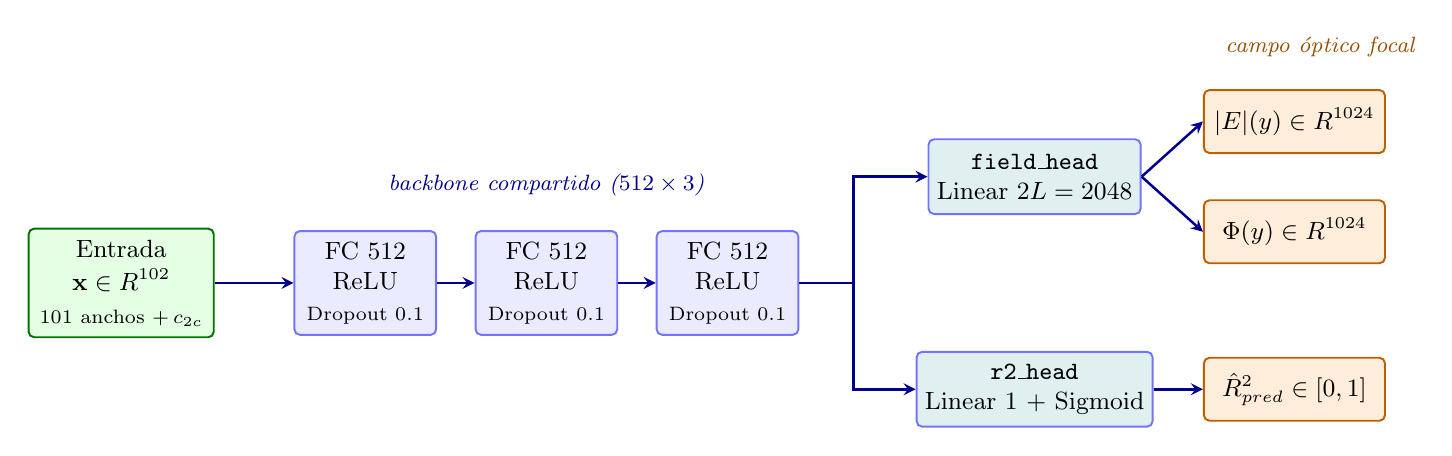
\begin{tikzpicture}[>=stealth, font=\small,
    box/.style={draw=blue!55, line width=0.7pt, rounded corners=2pt, fill=blue!8,
                minimum height=1.05cm, align=center, inner sep=4pt},
    head/.style={draw=blue!55, line width=0.7pt, rounded corners=2pt, fill=teal!12,
                 minimum height=0.95cm, align=center, inner sep=3pt},
    outbox/.style={draw=orange!75!black, line width=0.7pt, rounded corners=2pt, fill=orange!14,
                minimum height=0.8cm, align=center, inner sep=3pt},
    flow/.style={->, line width=0.9pt, draw=blue!55!black}]

  %% --- Entrada ---
  \node[box, fill=green!10, draw=green!45!black, minimum width=2.1cm] (in) at (0,0)
      {Entrada\\[1pt] $\mathbf{x}\in\mathbb{R}^{102}$\\[1pt] \scriptsize 101 anchos $+\,c_{2c}$};

  %% --- Backbone (3 capas ocultas) ---
  \node[box, minimum width=1.8cm] (h1) at (3.1,0) {FC $512$\\ ReLU\\ \scriptsize Dropout $0.1$};
  \node[box, minimum width=1.8cm] (h2) at (5.4,0) {FC $512$\\ ReLU\\ \scriptsize Dropout $0.1$};
  \node[box, minimum width=1.8cm] (h3) at (7.7,0) {FC $512$\\ ReLU\\ \scriptsize Dropout $0.1$};

  \draw[flow] (in) -- (h1);
  \draw[flow] (h1) -- (h2);
  \draw[flow] (h2) -- (h3);

  \node[font=\footnotesize\itshape, text=blue!55!black] at (5.4,1.25)
      {\textit{backbone} compartido ($512\times 3$)};

  %% --- Ramificación en dos cabezas ---
  \coordinate (branch) at (9.3,0);
  \draw[line width=0.9pt, draw=blue!55!black] (h3.east) -- (branch);

  \node[head, minimum width=2.2cm] (field) at (11.6,1.35) {\texttt{field\_head}\\ Linear $2L=2048$};
  \node[head, minimum width=2.2cm] (r2h)   at (11.6,-1.35) {\texttt{r2\_head}\\ Linear $1$ $+$ Sigmoid};

  \draw[flow] (branch) |- (field.west);
  \draw[flow] (branch) |- (r2h.west);

  %% --- Salidas ---
  \node[outbox, minimum width=2.3cm] (amp) at (14.9,2.05) {$|E|(y)\in\mathbb{R}^{1024}$};
  \node[outbox, minimum width=2.3cm] (pha) at (14.9,0.65) {$\Phi(y)\in\mathbb{R}^{1024}$};
  \node[outbox, minimum width=2.3cm] (r2)  at (14.9,-1.35) {$\hat{R}^2_{\text{pred}}\in[0,1]$};

  \draw[flow] (field.east) -- (amp.west);
  \draw[flow] (field.east) -- (pha.west);
  \draw[flow] (r2h.east)   -- (r2.west);

  %% --- Etiquetas de agrupación de salidas ---
  \node[font=\footnotesize\itshape, text=orange!60!black, align=left, anchor=west]
      at (13.9,3.0) {campo óptico focal};

\end{tikzpicture}
}
    \caption{Arquitectura del surrogate MLP multi-salida. El vector geométrico
    $\mathbf{x}\in\mathbb{R}^{102}$ atraviesa un \textit{backbone} de tres capas totalmente conectadas de $512$ unidades (ReLU $+$ \textit{dropout} $0.1$), del que se desprenden dos cabezas: \texttt{field\_head}, que reconstruye la amplitud y la fase del campo focal ($2L=2048$ salidas), y \texttt{r2\_head}, que produce el escalar $\hat{R}^2_{\text{pred}}$ con activación sigmoide. El \textit{backbone} compartido
    induce una representación interna útil para ambas tareas.}
    \label{fig:mlp_arquitectura}
\end{figure}

El modelo tiene ${\sim}1.63$ millones de parámetros (Figura~\ref{fig:mlp_arquitectura}). La función de pérdida combina los tres términos con pesos relativos:

\begin{equation}
    \mathcal{L} = w_{\text{amp}}\,\text{MSE}(|E|) + w_{\Phi}\,\text{MSE}(\Phi)
    + w_{R^2}\,\text{MSE}(\hat{R}^2_{\text{pred}}),
    \label{eq:loss_mvp}
\end{equation}

\noindent con $w_{\text{amp}} = w_{\Phi} = 1.0$ y $w_{R^2} = 10.0$ (el término escalar requiere mayor peso por su menor magnitud). El optimizador es Adam con tasa de aprendizaje $10^{-3}$ y \textit{ReduceLROnPlateau}, con \textit{early stopping} (paciencia 30 épocas) sobre la pérdida de validación.

\subsubsection{Inclusión de la Cabeza Escalar $\hat{R}^2_{\text{pred}}$}\label{subsubsec:r2head}

Idealmente, el criterio de éxito se calcularía propagando el campo predicho a una región longitudinal y ajustando la parábola, como hace el extractor de \textit{features} del simulador. Se implementó dicha propagación mediante el método del espectro angular (\textit{Angular Spectrum Method}), validándola con campos reales (correlación $0.84$ con el $R^2$ real del archivo HDF5). Sin embargo, al alimentarla con el campo \textit{predicho} por el subrogado, la correlación cae a ${\sim}0.20$: la propagación FFT amplifica los errores de fase del subrogado. Por ello se añadió $\hat{R}^2_{\text{pred}}$ como salida escalar supervisada directamente, evitando la propagación en la trayectoria de optimización.

\subsubsection{Ponderación por Muestra}

Para reforzar el aprendizaje en la región de alto rendimiento, se asignó un peso por muestra (\texttt{sample\_weight}) según la banda de $R^2$ y el origen del dato. Las simulaciones de las iteraciones de confirmación con $R^2 \geq 0.90$ reciben el peso máximo, las de $[0.85, 0.90)$ un peso intermedio-alto, y la masa central ($R^2$ bajo) peso unitario. A diferencia del primer enfoque, esta ponderación no busca corregir desbalance de clases, pues ya no hay clasificación, sino enfatizar la fidelidad del campo predicho donde más importa.

% --------------------------------------------------
\subsection{Datos y Particiones}\label{subsec:datos_mvp}

Las particiones del dataset ($1{,}110$ simulaciones estratificadas por $R^2$ con semilla $42$ en $781/161/168$, con las geometrías confirmadas forzadas a entrenamiento) se definieron en la Sección~\ref{subsec:consolidacion}. Aquí solo se añade el pre-procesamiento propio del modelo. La entrada se normaliza con un escalador Min-Max ajustado únicamente en entrenamiento, y la fase se escala por la desviación estándar agregada de todos sus valores en el conjunto de entrenamiento (${\sim}12.4$~rad, frente al promedio por simulación de $10.2$~rad reportado en el EDA), de modo que sus residuales sean comparables en magnitud a los de la amplitud durante la optimización. Esta normalización de la fase explica que las magnitudes internas de la pérdida (Figura~\ref{fig:training_curves}) difieran de los errores expresados en radianes de la Tabla~\ref{tab:surrogate_metrics}.

% --------------------------------------------------
\subsection{Evaluación del Subrogado}\label{subsec:eval_surrogate}

El entrenamiento converge en ${\sim}47$ épocas (${\sim}0.5$~min en CPU, dado el tamaño reducido del dataset). La Figura~\ref{fig:training_curves} muestra la evolución de la pérdida.

\begin{figure}[H]
    \centering
    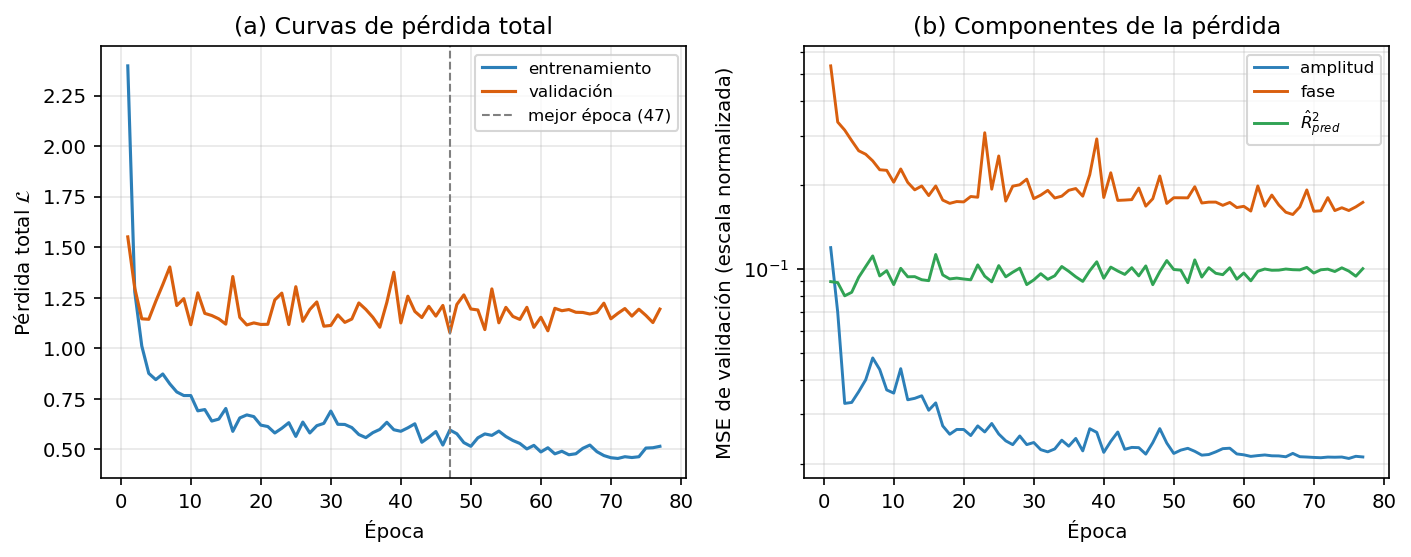
\includegraphics[width=\textwidth]{Figuras/fig_training_curves.png}
    \caption{Dinámica de entrenamiento del surrogate. (a)~Pérdida total de entrenamiento y validación por época: la validación alcanza su mínimo en la época $47$ (línea discontinua) y se estabiliza, mientras la de entrenamiento sigue descendiendo; el
    \textit{early stopping} detiene el ajuste $30$ épocas después. (b)~Componentes de la pérdida de validación en escala normalizada: la fase domina en magnitud y es el término más inestable, mientras la amplitud converge a un valor bajo y estable.}
    \label{fig:training_curves}
\end{figure}

Las curvas revelan dos rasgos coherentes con la naturaleza del problema. Primero, existe un margen de generalización moderado: la pérdida de entrenamiento desciende muy por debajo de la de validación, pero esta última no aumenta tras su mínimo, sino que se estabiliza. El \textit{dropout} y el \textit{early stopping} en la época $47$ contienen el sobreajuste sin necesidad de regularización adicional, un resultado esperable dado el tamaño reducido del dataset frente a la dimensión de la salida. Segundo, la descomposición por componente (panel b) confirma lo anticipado en el EDA: la fase es la fuente dominante e inestable de error, sus picos corresponden a la minoría de geometrías con frentes de onda de gran excursión, mientras que la amplitud y $\hat{R}^2_{\text{pred}}$ se aprenden de forma estable. La Tabla~\ref{tab:surrogate_metrics}
resume las métricas finales en el conjunto de prueba.

\begin{table}[H]
\centering
\small
\begin{tabular}{lcc}
\toprule
\textbf{Métrica (test)} & \textbf{Modelo final} & \textbf{5 semillas} \\
                        & \textbf{(semilla 42)} & \textbf{(media $\pm\,\sigma$)} \\
\midrule
MSE amplitud (media)                          & 0.026        & $0.035 \pm 0.005$ \\
MSE fase (media / mediana, rad$^2$)           & 30.1 / 16.4  & $35.6 \pm 4.3$ \\
RMSE de $\hat{R}^2_{\text{pred}}$             & 0.29         & $0.28 \pm 0.02$ \\
Corr.\ $\hat{R}^2_{\text{pred}}$ vs $R^2_{\text{real}}$ & $+0.29$ & $+0.31 \pm 0.02$ \\
\bottomrule
\end{tabular}
\caption{Métricas del surrogate MLP multi-salida en el conjunto de prueba. La columna, 5 semillas, reporta media$\,\pm\,\sigma$ de reentrenar el modelo con cinco semillas distintas; el modelo final (semilla 42) es el desplegado en el optimizador.}
\label{tab:surrogate_metrics}
\end{table}

La última columna descarta que estas cifras dependan de una inicialización afortunada: al reentrenar con cinco semillas, la correlación $\hat{R}^2_{\text{pred}}$--$R^2_{\text{real}}$ se mantiene estable en $+0.31 \pm 0.02$ y el resto de métricas varía poco, de modo que el ordenamiento de candidatos es robusto a la semilla.

La amplitud, que determina directamente la forma del lóbulo focal, se predice con error bajo: un MSE medio de $0.026$ sobre un vector acotado en $[0,1]$ equivale a un RMSE de ${\approx}0.16$. La fase es intrínsecamente más difícil, como anticipó el EDA (Sección~\ref{subsec:campo_focal}): su MSE medio de $30$~rad$^2$ corresponde a un RMSE de ${\approx}5.5$~rad.

Calificar esta reconstrucción de aceptable no es una concesión vaga, sino una afirmación cuantificada en tres sentidos. (i)~Ese RMSE representa menos de la mitad de la desviación estándar agregada de la señal de fase (${\sim}12.4$~rad) y alrededor del $15\%$ de su rango dinámico (${\sim}36$~rad): el error es una fracción de la variabilidad que el modelo debe capturar. (ii)~La media del error está inflada por una minoría de casos difíciles, de modo que en la simulación típica la fase se reproduce con fidelidad y solo una cola de geometrías concentra el error, como muestran los picos del panel~(b) de la Figura~\ref{fig:training_curves}. (iii)~La estructura del frente de onda se conserva, lo que basta para que el campo predicho ordene candidatos, aunque no con la fidelidad absoluta que exigiría propagarlo numéricamente; este residual de fase es precisamente lo que desvirtúa la propagación por espectro angular y lo que motivó la cabeza escalar $\hat{R}^2_{\text{pred}}$ (Sección~\ref{subsubsec:r2head}) en lugar de derivar el $R^2$ del campo. En esa línea, la correlación entre $\hat{R}^2_{\text{pred}}$ y el $R^2$ real es moderada y positiva ($\approx +0.29$), suficiente para ordenar geometrías candidatas pero no para predecir su valor absoluto con precisión.

La Figura~\ref{fig:surrogate_overlay} ilustra cualitativamente esta evaluación sobre un enfocador representativo del conjunto de prueba: el surrogate reproduce la envolvente de la amplitud y la curvatura global de la fase, las características que gobiernan la calidad de enfoque, aunque suaviza las oscilaciones transversales finas, lo que es coherente con el bajo MSE de amplitud y el carácter aceptable de la fase ya discutidos.

\begin{figure}[H]
    \centering
    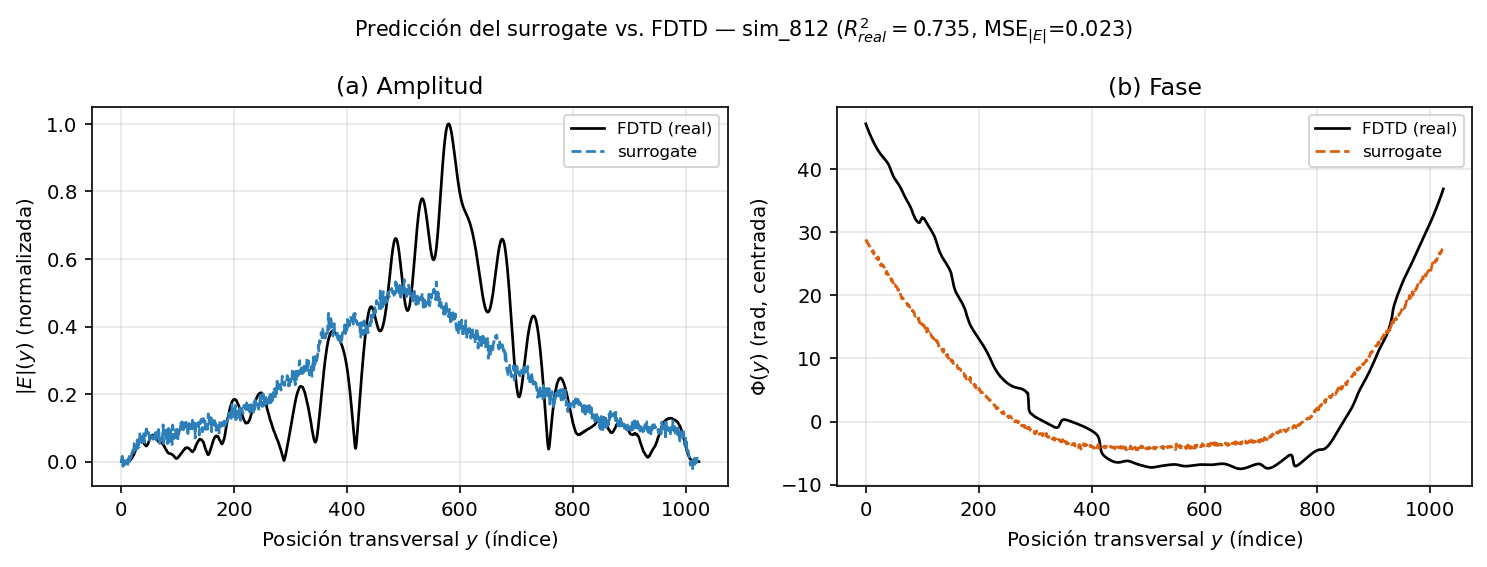
\includegraphics[width=\textwidth]{Figuras/fig_surrogate_overlay.png}
    \caption{Predicción del surrogate (línea discontinua) frente al campo real de FDTD (línea continua) para un enfocador representativo del conjunto de prueba. (a)~La amplitud predicha sigue la envolvente del perfil real; (b)~la fase predicha reproduce la curvatura global del frente de onda. El surrogate captura la estructura relevante
    para el enfoque y suaviza el detalle de alta frecuencia.}
    \label{fig:surrogate_overlay}
\end{figure}

\subsubsection{Limitación Conocida}

En la zona de alto rendimiento ($R^2_{\text{real}} \geq 0.7$) la correlación se debilita e incluso se invierte: el surrogate sobreestima en esa región. En consecuencia, un valor $\hat{R}^2_{\text{pred}}$ elevado no garantiza un $R^2$ real alto, y la confirmación por FDTD sigue siendo indispensable para verificar el criterio de éxito. Esta limitación condiciona el diseño del optimizador (Sección~\ref{sec:optimizacion}), que no puede confiar ciegamente en el escalar predicho y debe restringirse a vecindarios del manifold de geometrías ya validadas.
